\section{Nocturia}

In this part the studies on nocturia are discussed. 

\subsection{What is nocturia?}

Waking at night to void is known as nocturia. It is a common condition experienced by both male and female with profound impact on patient's health, \gls{QoL} (Quality of Life) and economic condition. Nocturia is perceived as a symptom of many disorders. ~\textcite{nocturia_symptom} ~\textcite{nocturia_misjudged}
The underlying pathophysiologic process of nocturnia comprises four main conditions. 

\begin{enumerate}
	\item{Global polyuria}
	\item{Nocturnal polyuria}
	\item{Nocturnal urine overproduction}
	\item{Decreased nocturnal bladder capacity}
\end{enumerate}

\subsection{Impact of nocturia}

Nocturia causes sleep fragmentation and disruption and may result in daytime sleepiness, tiredness, mood changes and cognitive dysfunction with poor concentration and performance. ~\textcite{nocturia_mgmt} 


The lack of sleep caused by excessive nighttime voiding leads to lower energy levels (vitality), impaired work-related productivity, and reduced \gls{QoL}. Nocturia also has been known to be linked to a heightened risk for traffic accidents, morbidity, mortality, and significant health costs to both the patient and the physician.  ~\textcite{Nocturia_productivity}

\subsection{Assessment of nocturia}

The formula for calculating \gls{NPi} (Nocturnal Polyuria index) is \gls{NUV} (Nocturnal urinary volume) divided by 24-h urine volume. \\
The formula for calculating nocturnal index is \gls{NUV} divided by \gls{MVV} (Maximum voided volume). \\
The formula for calculating nocturnal bladder capcity index is \\ \verb|(nocturnal index - 1) - (#nightly voids)|

\begin{center}
	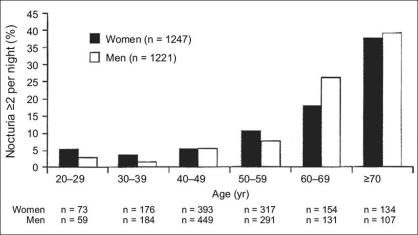
\includegraphics[width=.8\textwidth,keepaspectratio]{nocturia.jpg}
	\captionof{figure}{Algorithm for investigating nocturia}
	\label{fig:alg_nocturia}
\end{center}

\subsection{Global polyuria}

Polyuria is a continuous overproduction of urnine not limited to sleep hours and defined as 24-h urine output of more than 40 ml/kg. Polyuria is associated with increased urinary frequency during both daytime and nighttime. The most common causes are \gls{DI} (Diabetes Insipidus), diabetes mellitus and primary thirst disorders. \\

\gls{DI} the less common form of diabetes is a water balance disorder. The inappropriate excretion of urine may lead to polydipsia (thirst disorder). In people with \gls{DI} the pituitary gland produces a normal amount of intidiuretic hormone but the kidneys do not respond appropriately to it. Diagnosis is made by overnight water deprivation to determine wether the urine becomes more concentrated. If the first morning void is not highly concentrated, \gls{DI} is diagnosed. If the water deprivation test is normal in a person experiencing polyuria, the diagnosis is a thirst disorder.  \textcite{polyuria_vs_overactive_bladder}

